\documentclass[tikz, border=0pt]{standalone}
\usetikzlibrary{patterns,angles,quotes}

\begin{document}
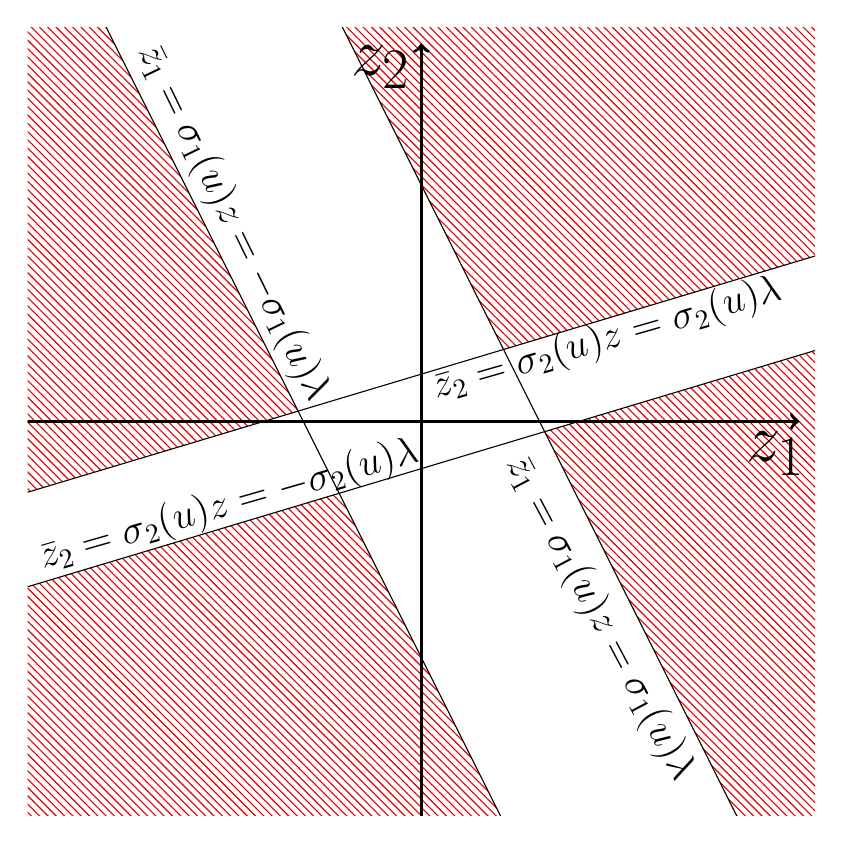
\begin{tikzpicture}
    % Draw and hatch a rectangle
    % \draw[fill, pattern=north west lines, pattern color=blue] (0,0) rectangle (4,2);

    % % Draw and hatch a custom polygon
    % \draw[fill, pattern=crosshatch dots, pattern color=red] (5,0) -- (7,3) -- (9,1) -- cycle;

    % % Draw and hatch a circle
    % \draw[fill, pattern=grid, pattern color=green!50!black] (12,1) circle (1.5);

    % \coordinate (A) at (2,0);
    % \coordinate (B) at (0,0);
    % \coordinate (C) at (1,1);

    % \draw (A) -- (B) -- (C); % Draw the lines forming the angle

    % \pic [draw,fill,  pattern=grid, pattern color=green!50!black] {angle = A--B--C}; % Draw and label the angle arc

    % \coordinate (D) at (3,0);
    % \coordinate (E) at (0,0);
    % \coordinate (F) at (1,2);
    
    % \draw (D) -- (E) -- (F);
    
    % \pic[draw, angle radius=1cm, "$\Vert$"] {angle = D--E--F}; % Use `$\Vert$` for double hash

   
    % Define the clipping region for the first quadrant
    \clip (-5,-5) rectangle (5,5);

    % Fill the region below y = 1/x
    \path[pattern=north west lines, pattern color=red!90!black] 
        (3.6/2.3,-0.3/2.3) -- (5.2,0.95) -- (5.2,-7.4) -- cycle;

    \path[pattern=north west lines, pattern color=red!90!black] 
        (-3.6/2.3,0.3/2.3) -- (-5.2,-0.95) -- (-5.2,+7.4) -- cycle;


    \path[pattern=north west lines, pattern color=red!90!black] 
        (24/23,21/23) -- (8.2,.3*10.2) -- (-4,11) -- cycle;

    \path[pattern=north west lines, pattern color=red!90!black] 
        (-24/23,-21/23) -- (-8.2,-.3*10.2) -- (4,-11) -- cycle;

    % Draw the main curve and axes
    \draw[domain=-5.2:5.2] plot[samples=100] (\x, {0.3*(\x-2)}) node[right, rotate=16] at (24/23-1,21/23-0.54) {\Large $\bar{z}_2=\sigma_2(u)z=\sigma_2(u)\lambda$};
    \draw[domain=-5.2:5.2] plot[samples=100] (\x, {0.3*(\x+2)}) node[right, rotate=16] at (24/23-6,21/23-2.7) {\Large $\bar{z}_2=\sigma_2(u)z=-\sigma_2(u)\lambda$} ;

    \draw[domain=-5.2:5.2] plot[samples=100] (\x, {3-2*\x}) node[right, rotate=-64] at (3.6/2.3-5.1,-0.3/2.3+5) {\Large $\bar{z}_1=\sigma_1(u)z=-\sigma_1(u)\lambda$} ;
    \draw[domain=-5.2:5.2] plot[samples=100] (\x, {-3-2*\x}) node[right, rotate=-62] at (-3.6/2.3+2.7,0.3/2.3-.5) {\Large $\bar{z}_1=\sigma_1(u)z=\sigma_1(u)\lambda$};

    
    \draw[->,very thick] (0-5.2,0) -- (4.8,0) node[below] at (4.5,0) {\Huge${z}_1$};
    \draw[->,very thick] (0,-5.2) -- (0,4.8) node[left] at (0,4.5) {\Huge${z}_2$};

    % \draw (2,-5.2) -- (2,5.2) node[right, rotate=90] at (1.8,3) {$\sigma(u)z_1=\lambda$};

    % \draw (-2,-5.2) -- (-2,5.2) node[right, rotate=90] at (-1.8,3) {$z_1=-\lambda$};

    % \draw (-5.2,2) -- (5.2,2) node[ rotate=0] at (3,1.8) {$z_2=\lambda$};


    
    % \draw (-5.2,-2) -- (5.2,-2) node[ rotate=0] at (3,-1.8) {$z_2=-\lambda$};
    % Draw a point to show the boundary starts at x=1
    % \filldraw[black] (1,1) circle (2pt);
    % \node[below] at (1,0) {1};
    % \node[left] at (0,1) {1};
    
    % Add the label
    % \node[above, right, blue] at (3,0.5) {$y = 1/x$};


\end{tikzpicture}
\end{document}